\section{eo\-Selective\-Populator$<$ EOT $>$ Class Template Reference}
\label{classeo_selective_populator}\index{eoSelectivePopulator@{eoSelectivePopulator}}
Selective\-Populator an eo\-Poplator that uses an {\bf eo\-Select\-One}{\rm (p.\,\pageref{classeo_select_one})} to select guys.  


{\tt \#include $<$eo\-Populator.h$>$}

Inheritance diagram for eo\-Selective\-Populator$<$ EOT $>$::\begin{figure}[H]
\begin{center}
\leavevmode
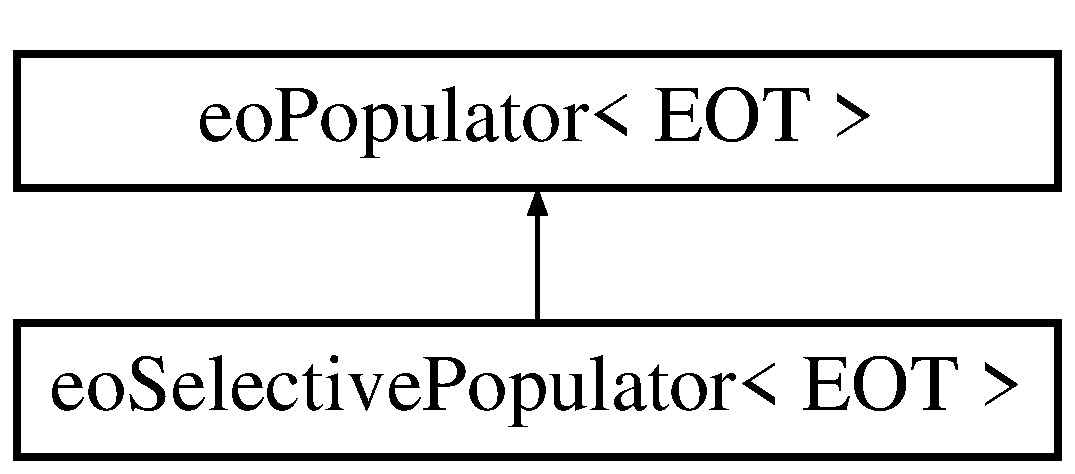
\includegraphics[height=2cm]{classeo_selective_populator}
\end{center}
\end{figure}
\subsection*{Public Member Functions}
\begin{CompactItemize}
\item 
{\bf eo\-Selective\-Populator} (const {\bf eo\-Pop}$<$ {\bf EOT} $>$ \&\_\-pop, {\bf eo\-Pop}$<$ {\bf EOT} $>$ \&\_\-dest, {\bf eo\-Select\-One}$<$ {\bf EOT} $>$ \&\_\-sel)\label{classeo_selective_populator_a0}

\item 
const {\bf EOT} \& {\bf select} ()\label{classeo_selective_populator_a1}

\begin{CompactList}\small\item\em the select method actually selects one guy from the src pop \item\end{CompactList}\end{CompactItemize}
\subsection*{Private Attributes}
\begin{CompactItemize}
\item 
{\bf eo\-Select\-One}$<$ {\bf EOT} $>$ \& {\bf sel}\label{classeo_selective_populator_r0}

\end{CompactItemize}


\subsection{Detailed Description}
\subsubsection*{template$<$class EOT$>$ class eo\-Selective\-Populator$<$ EOT $>$}

Selective\-Populator an eo\-Poplator that uses an {\bf eo\-Select\-One}{\rm (p.\,\pageref{classeo_select_one})} to select guys. 

Supposedly, it is passed the initial population. 



Definition at line 184 of file eo\-Populator.h.

The documentation for this class was generated from the following file:\begin{CompactItemize}
\item 
eo\-Populator.h\end{CompactItemize}
